\chapter[Arquitetura de Integração]{Arquitetura de Integração}

A arquitetura de integração contém aspectos da solução de eletrônica, energia, estrutura e software e está representado na figura \ref{fig:arq_integracao}. Para a alimentação dos componentes no dispositivo a solução de energia projetou uma fonte de 12V e 15A para realizar a alimentação dos \textit{drivers} do motor DC, do motor de passo, do solenoide e do atuador. Para o restante dos componentes eletrônicos será utilizado um regulador de tensão de 12V para uma saída de 5V e 8A, representado no diagrama como a fonte de 5V e 8 A.

A solução eletrônica está representado pelos subsistemas do modulo de medição, módulo de interação e módulo de acionamento dos atuadores. A conexão entre esse módulos é feita pela central de controle representada pelo microprocessador e microcontroladores. Para comunicação entre a solução eletrônica e o \textit{backend} da arquitetura de software, representado pelos módulos de exposição, serviços negociais, armazenamento de dados e fila, é utilizado os protocolos de comunicação MQTT e HTTP. O \textit{frontend} é representado pelo módulo de interação e se comunica com o \textit{backend}, em específico o módulo de exposição, por meio do protocolo HTTP.

\begin{landscape}
\begin{figure}[!htb]
    \centering
    \vspace{2cm}
    \hspace{-2cm}
    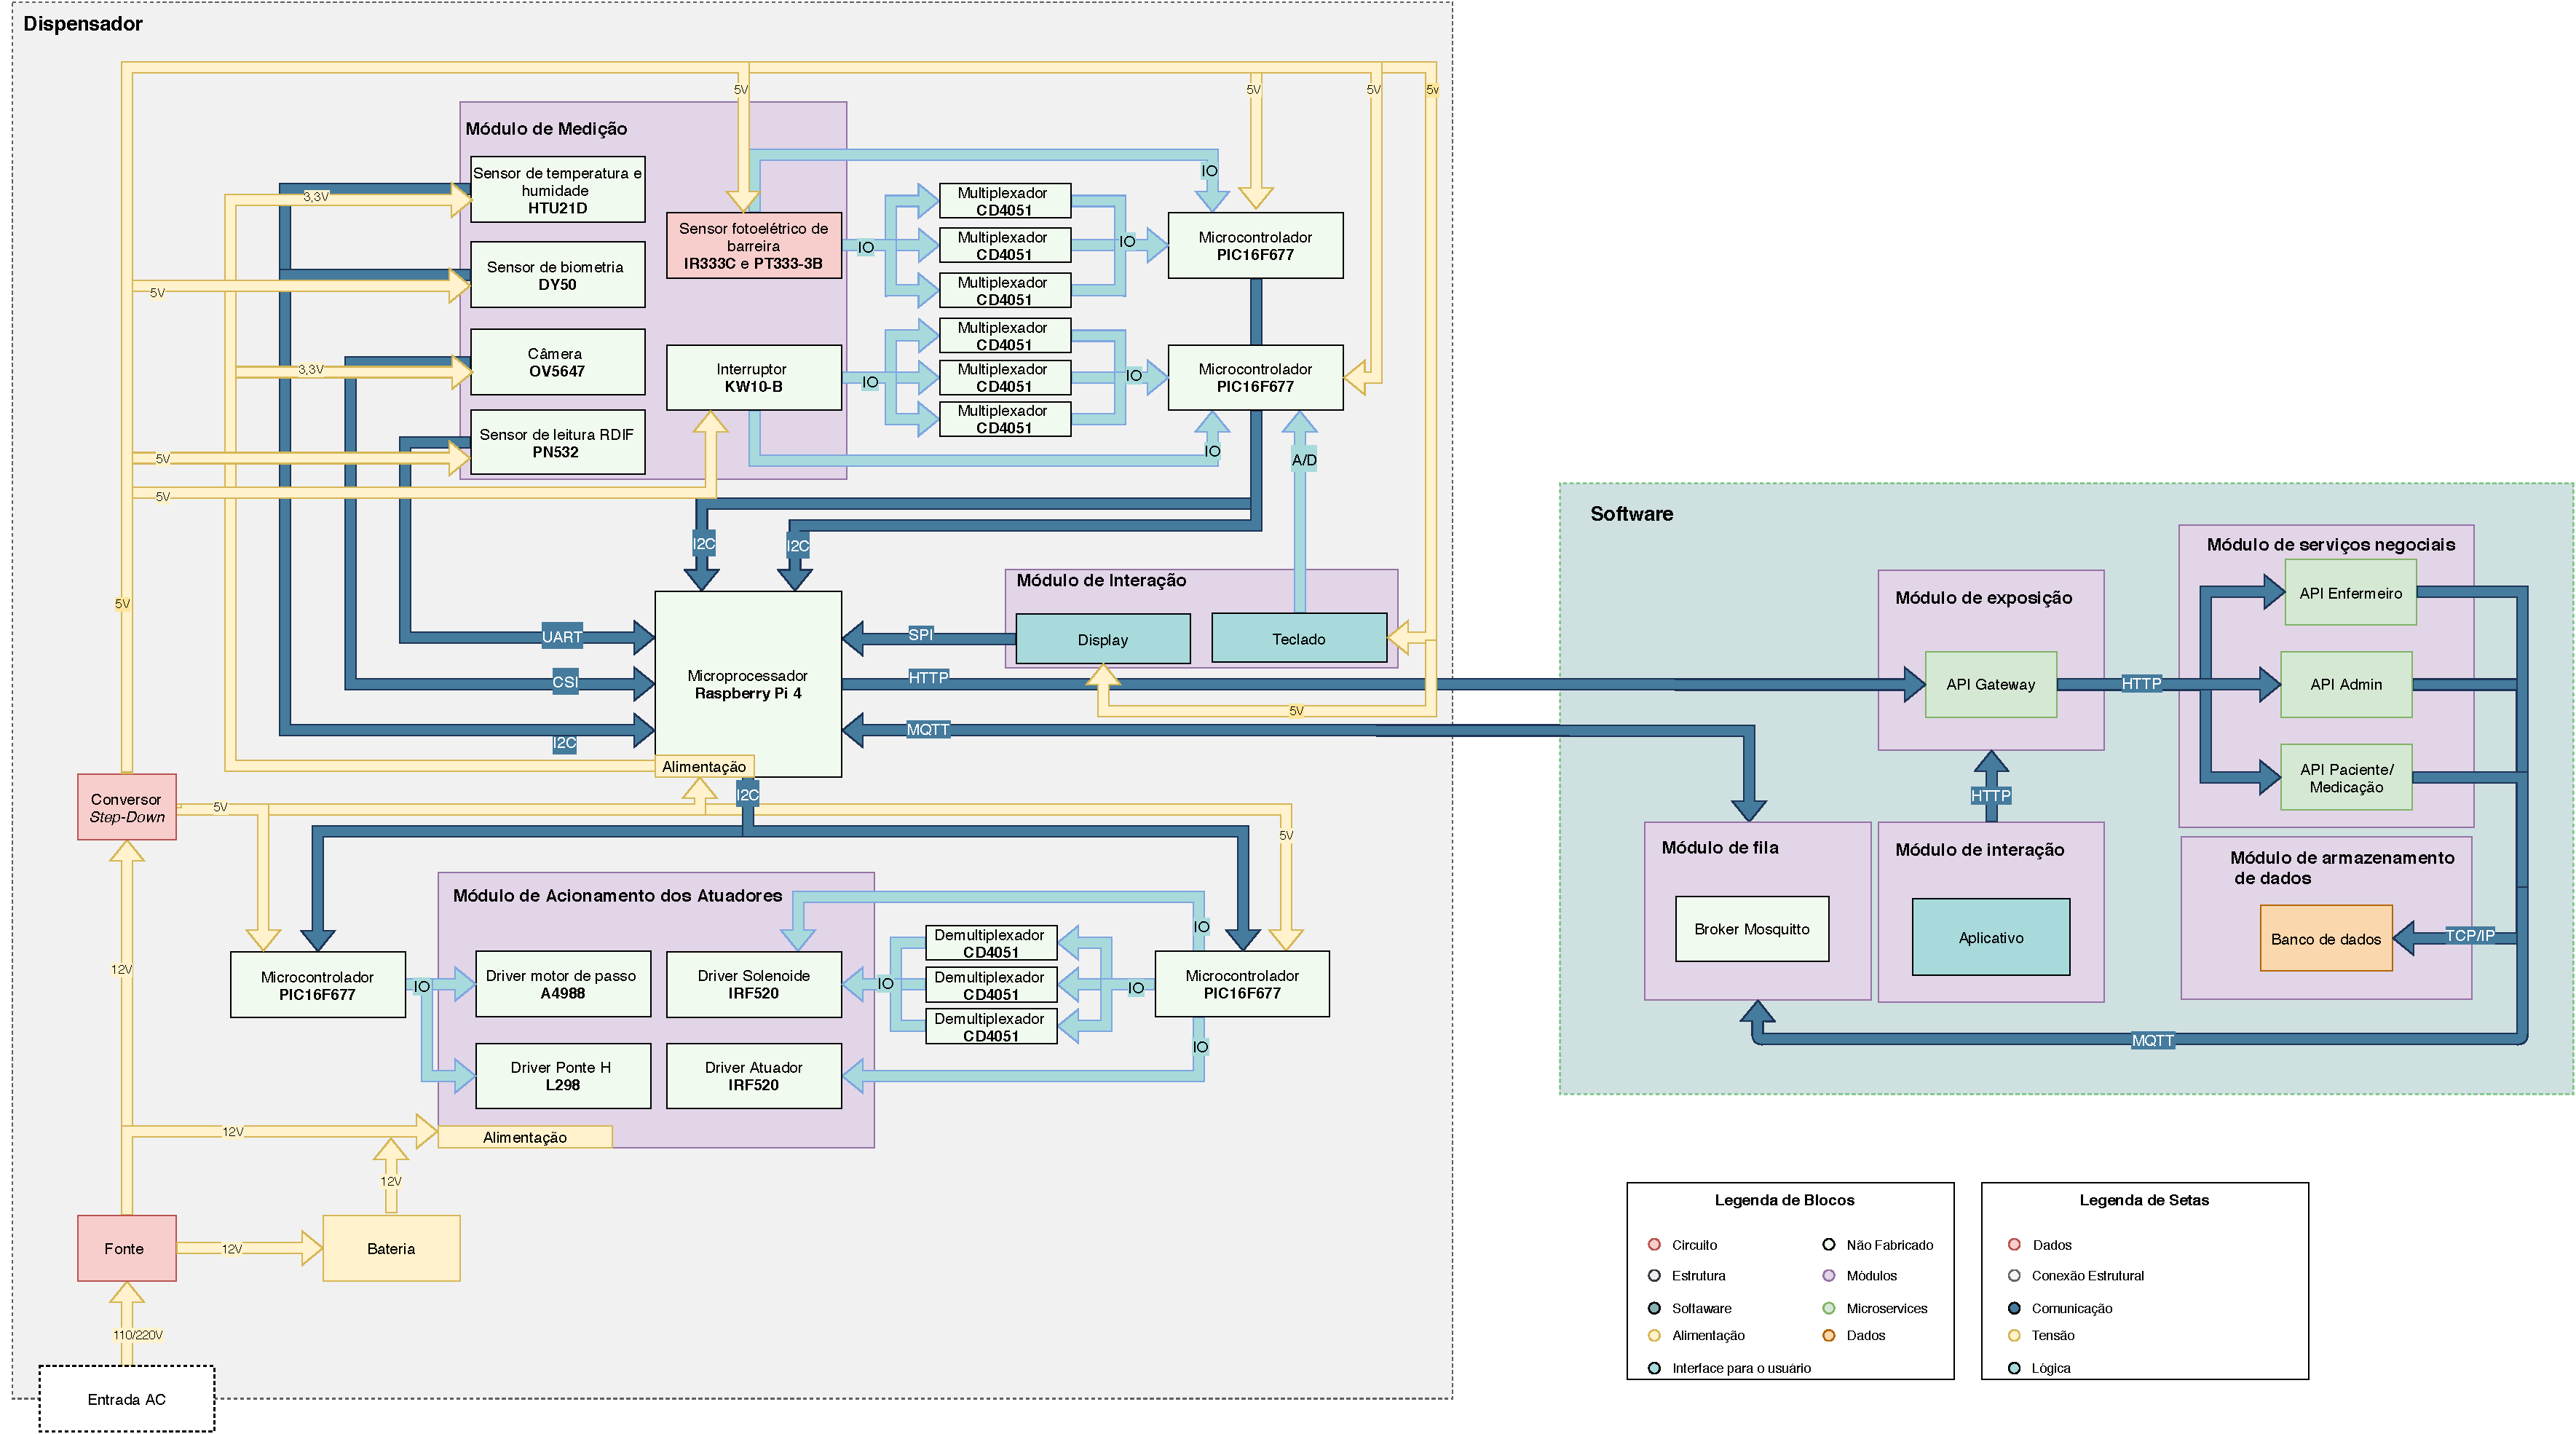
\includegraphics[width=1.5\textwidth, height=2\textheight,keepaspectratio]{figuras/integracao_geral.pdf}
    \vspace{-5pt}
    \caption{Arquitetura de Integração}
    \label{fig:arq_integracao}
\end{figure}
\end{landscape}
